% =====================================================================
% Guia: geometria y malla del sedimentador con Gmsh para OpenFOAM
% Compilar con pdflatex, xelatex o lualatex (dos pasadas):  xelatex guia_sedimentador.tex
% Figuras requeridas en la misma carpeta: fig_geometria.png, fig_malla.png
% =====================================================================
\documentclass[10pt,a4paper]{article}

\usepackage{iftex}
\ifPDFTeX
  % pdfLaTeX
  \usepackage[utf8]{inputenc}
  \usepackage[T1]{fontenc}
  \IfFileExists{lmodern.sty}{\usepackage{lmodern}}{}
  \usepackage[spanish,es-noshorthands]{babel}
\else
  % XeLaTeX / LuaLaTeX
  \usepackage{fontspec}
  \usepackage{polyglossia}
  \setdefaultlanguage{spanish}
\fi
\usepackage[margin=2cm]{geometry}
\usepackage{graphicx}
\usepackage{booktabs}
\usepackage{tabularx}
\usepackage{array}
\usepackage{xcolor}
\usepackage{listings}
\usepackage{enumitem}
\usepackage{caption}
\usepackage[colorlinks=true,linkcolor=blue!50!black,urlcolor=blue!50!black]{hyperref}

\setlist{itemsep=1pt,topsep=3pt,parsep=0pt}
\setlength{\parindent}{0pt}
\setlength{\parskip}{4pt}
\captionsetup{font=small,labelfont=bf}
\renewcommand{\arraystretch}{1.15}
\newcolumntype{L}{>{\raggedright\arraybackslash}X}

% Codigo en linea (admite _ { } # sin escapar)
\newcommand{\code}[1]{\texttt{\detokenize{#1}}}

% Bloques de codigo
\lstset{
  basicstyle=\ttfamily\footnotesize,
  columns=fullflexible,
  keepspaces=true,
  frame=single,
  rulecolor=\color{black!25},
  backgroundcolor=\color{black!3},
  xleftmargin=0pt,
  aboveskip=4pt,
  belowskip=2pt,
  breaklines=true,
  upquote=true
}
\ifPDFTeX
\lstset{
  literate={á}{{\'a}}1 {é}{{\'e}}1 {í}{{\'i}}1 {ó}{{\'o}}1 {ú}{{\'u}}1
           {Á}{{\'A}}1 {É}{{\'E}}1 {Í}{{\'I}}1 {Ó}{{\'O}}1 {Ú}{{\'U}}1
           {ñ}{{\~n}}1 {Ñ}{{\~N}}1 {×}{{$\times$}}1 {…}{{...}}1
}
\fi

\newcommand{\paso}[1]{\par\smallskip\textbf{#1}}

\title{Caso base: geometría y malla del sedimentador\\con Gmsh para OpenFOAM}
\author{Ayudantía UCC}
\date{16 de octubre de 2026}

\begin{document}
\maketitle
\vspace{-1.2em}

%---------------------------------------------------------------------
\section{Objetivo y archivos}
Este caso base construye con Gmsh una malla 100\,\% hexaédrica del sedimentador (tolva más cuerpo) y la deja lista para OpenFOAM, siguiendo dos caminos que terminan en 37 volúmenes de malla estructurada.

\begin{tabularx}{\textwidth}{@{}l l L r@{}}
\toprule
Archivo & Método & Cómo arma la geometría & Líneas \\
\midrule
\code{mallaBase3D_v0.geo} & A: explícito & Puntos, líneas, superficies y volúmenes definidos uno por uno & 345 \\
\code{mallaBase3D_v1.geo} & B: loft & Una macro crea las secciones y \code{ThruSections} las une & 103 \\
\bottomrule
\end{tabularx}

Ambos usan el kernel OpenCASCADE, definen un único tamaño de celda (\code{tamanoDeCelda = 0.1} m), tienen las mismas cotas y terminan con los mismos grupos físicos: \code{internalMesh} y \code{top}.

\textbf{Requisitos:}
\begin{itemize}
  \item Gmsh 4.x (los scripts se probaron con 4.15.2).
  \item OpenFOAM con \code{gmshToFoam} y \code{checkMesh}.
  \item Ambos \code{.geo} en la misma carpeta de trabajo.
\end{itemize}

Para probar un script sin escribir nada en disco: \code{gmsh mallaBase3D_v1.geo} abre la interfaz gráfica; luego \emph{Mesh $\rightarrow$ 3D}. En la consola aparecen los mensajes de \code{Printf} (secciones 3 y 4).

%---------------------------------------------------------------------
\section{La geometría}
La pieza es una tolva que se abre desde un fondo de $0.5 \times 0.5$ m hasta un cuerpo prismático, que a su vez se ensancha en $x$. Se describe con \textbf{6 secciones horizontales} ($k = 1$ a 6) unidas por \textbf{5 tramos}:
\begin{enumerate}
  \item Tramo 1 ($z = 0$ a 3 m): la tolva, de $0.5 \times 0.5$ m a la sección completa.
  \item Tramo 2 ($z = 3$ a 4.60 m): cuerpo vertical.
  \item Tramo 3 ($z = 4.60$ a 5.65 m): la cara de aguas abajo se inclina y el ancho en $x$ crece 0.7485 m.
  \item Tramos 4 y 5 ($z = 5.65$ a 6.65 m y hasta el tope): cuerpo vertical con el ancho ya ensanchado.
\end{enumerate}

Sobre todo el cuerpo ($z \geq 3$ m) se agrega una franja lateral de \textbf{0.18 m} en las cuatro caras, que se malla con 2 capas. Además, toda la pieza se desplaza 0.18 m en $x$ e $y$ para quedar en la misma posición que en el plano de AutoCAD respecto del origen $(0,0,0)$.

Las cotas son las mismas en los dos scripts:

\begin{tabularx}{\textwidth}{@{}L r@{}}
\toprule
Cota & Valor \\
\midrule
Ancho del cuerpo en $x$ e $y$ (tramos 1 a 3) & 4.45 m \\
Ancho en $x$ con el ensanche (tramos 4 y 5) & $4.45 + 0.7485 = 5.1985$ m \\
Altura total & 6.95 m \\
Altura del último tramo & 0.30 m \\
Fondo de la tolva (centrado en el cuerpo) & $0.5 \times 0.5$ m, de 1.975 a 2.475 m en $x$ e $y$ \\
Desplazamiento de 0.18 m & v0: \code{x0 = y0 = 0.18} en cada punto; v1: \code{Translate} al final del loft \\
\bottomrule
\end{tabularx}

\begin{figure}[h]
  \centering
  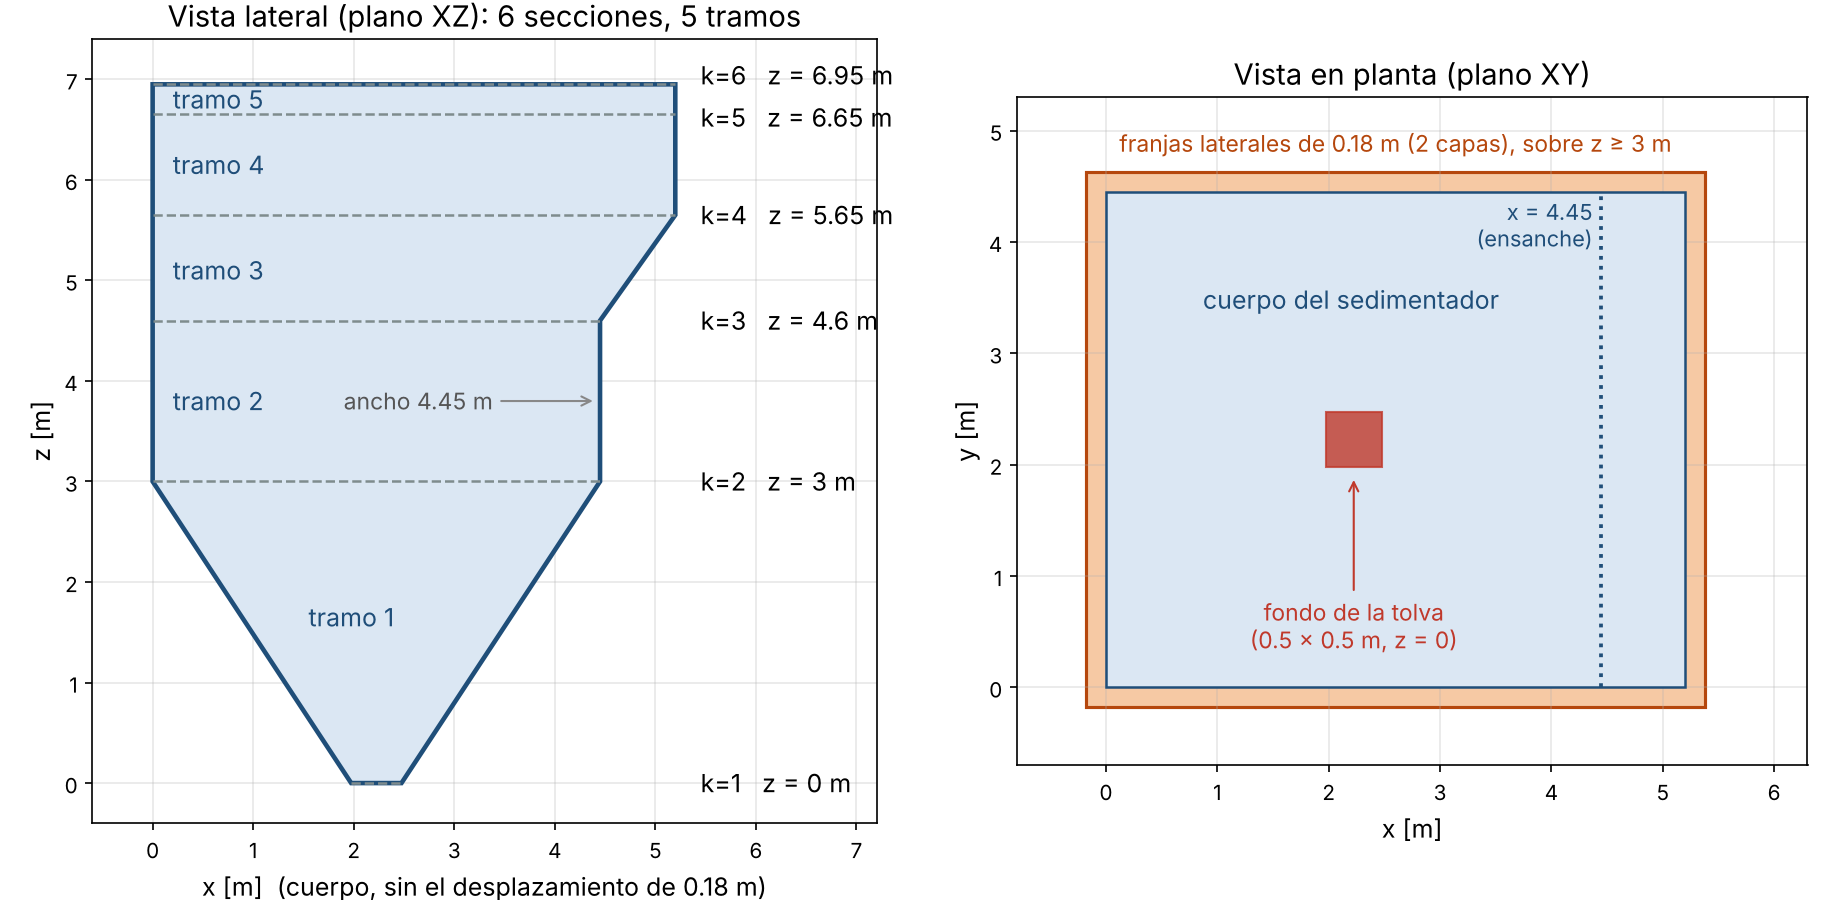
\includegraphics[width=\textwidth]{fig_geometria.png}
  \caption{Secciones y tramos. Las coordenadas del dibujo son las del cuerpo, antes del desplazamiento de 0.18 m; las franjas naranjas son el espesor lateral.}
\end{figure}

%---------------------------------------------------------------------
\section{Método A: geometría explícita (\texttt{mallaBase3D\_v0.geo})}
El método A construye cada entidad a mano, de abajo hacia arriba (puntos, líneas, superficies, volúmenes) y recién después impone la malla. Son siete pasos.

\paso{Paso 1. Kernel y origen.} Todas las coordenadas llevan \code{+x0}, \code{+y0}, \code{+z0}, así que mover la pieza es cambiar estas tres variables.
\begin{lstlisting}
SetFactory("OpenCASCADE");
x0 = 0.18;  y0 = 0.18;  z0 = 0;   // desplazamiento respecto del origen de AutoCAD
\end{lstlisting}

\paso{Paso 2. Puntos de la tolva.} Los puntos 1 a 4 son el fondo ($0.5 \times 0.5$ m, centrado) y los 5 a 8 la sección de $z = 3$ m. El cuarto valor (1.0) es un tamaño de celda que aquí no se usa, porque la malla se impone con \code{Transfinite}.
\begin{lstlisting}
Point(1) = {1.975+x0, 1.975+y0, 0+z0, 1.0};          // fondo
...
deltaV = 3;  deltaH = 1.975+0.5+1.975;               // 4.45 m
Point(5) = {x0, y0, z0+deltaV, 1.0};                 // tope de la tolva
\end{lstlisting}

\paso{Paso 3. Líneas, superficies y volumen de la tolva.} Las líneas 1 a 4 son el fondo, 5 a 8 el tope y 9 a 12 las aristas inclinadas. Cada cara sigue la cadena \code{Curve Loop} $\rightarrow$ \code{Plane Surface}, y el volumen sale de \code{Surface Loop} $\rightarrow$ \code{Volume}. El signo en un \code{Curve Loop} indica el sentido de recorrido (\code{-10} es la línea 10 al revés).
\begin{lstlisting}
Curve Loop(1) = {1, 2, 3, 4};   Plane Surface(1) = {1};   // fondo
Surface Loop(1) = {2, 6, 5, 1, 3, 4};
Volume(1) = {1};
\end{lstlisting}

\paso{Paso 4. Resolución de la tolva.} El número de nodos de una línea es \code{L / tamanoDeCelda + 1}. Gmsh \textbf{trunca} el resultado a entero: 4.45 m con celdas de 0.1 m da $44.5 + 1 = 45.5$, es decir 45 nodos y 44 celdas de 0.101 m (sección 5). Las verticales de la tolva miden 3 m: $30 + 1 = 31$ nodos. \code{Progression 1.02} hace que cada celda sea 1.02 veces la anterior en el sentido de la línea (de abajo hacia arriba), de modo que la tolva queda más fina en el fondo. \code{Transfinite Surface} y \code{Transfinite Volume} piden malla estructurada, y \code{Recombine} convierte los triángulos en cuadriláteros, que dan hexaedros.
\begin{lstlisting}
tamanoDeCelda = 0.1;
Longitud = 4.45;   resolucion1 = Longitud/tamanoDeCelda + 1;
Transfinite Curve {planoInferior[]} = resolucion1 Using Progression 1;
Longitud = 3;      resolucion2 = Longitud/tamanoDeCelda + 1;
Transfinite Curve {lineasVerticales[]} = resolucion2 Using Progression 1.02;
Transfinite Surface {tolva[]};  Recombine Surface {tolva[]};
Transfinite Volume{1};
\end{lstlisting}

\paso{Paso 5. Geometría del sedimentador.} Se repite el procedimiento para cuatro niveles ($z = 4.60$, 5.65, 6.65 y 6.95 m). Los niveles de 5.65 m en adelante suman \code{deltaH2 = 0.7485} m en $x$. La numeración queda así:

\begin{tabularx}{\textwidth}{@{}l l L@{}}
\toprule
Entidad & Tags & Qué son \\
\midrule
Puntos & 1--4, 5--8, 9--12, 13--16, 17--20, 21--24 & fondo, $z = 3$, 4.60, 5.65, 6.65 y 6.95 m \\
Líneas & 1--12, 13--28, 29--44 & tolva, bordes horizontales de los 4 niveles, verticales de cada tramo \\
Superficies & 1--6, 7--10, 11--26 & tolva, tapas horizontales, caras laterales de los 4 tramos \\
Volúmenes & 1, 2--5 & tolva, tramos 2 a 5 \\
\bottomrule
\end{tabularx}

\paso{Paso 6. Resolución del sedimentador.} Las verticales de cada tramo (\code{nivel1[]} a \code{nivel4[]}, de 1.6, 1.05, 1.0 y 0.3 m) se discretizan con la misma fórmula. Como las tapas 7 a 10 las comparten dos tramos vecinos, la malla coincide en la interfaz sin pegar nada.
\begin{lstlisting}
nivel1[] = {29:32};  h1 = 1.6;  R1 = h1/tamanoDeCelda + 1;
Transfinite Curve {nivel1[]} = R1 Using Progression 1;
Transfinite Surface {surfaceSedimentador[]};  Recombine Surface {surfaceSedimentador[]};
Transfinite Volume{volumenSedimentador[]};
\end{lstlisting}

\paso{Paso 7. Espesor lateral por extrusión.} Cada cara lateral se extruye 0.18 m con \code{Extrude} y 2 capas. Las caras se eligen con \code{Surface In BoundingBox {xmin, ymin, zmin, xmax, ymax, zmax}}, que \textbf{solo devuelve superficies que quedan completamente dentro de la caja}; por eso las cajas son delgadas ($\pm 0.001$ m) alrededor del plano buscado.
\begin{lstlisting}
aguasArriba[] = Surface In BoundingBox {0.179, -0.001, 0, 0.181, 5, 7};
Extrude {-L, 0, 0} { Surface{aguasArriba[]}; Layers {celdas}; Recombine; }
surperficies[] = {12, 16, 20, 24};                       // caras de aguas abajo
Extrude { L, 0, 0} { Surface{surperficies[]}; Layers {celdas}; Recombine; }
derecha[]   = Surface In BoundingBox {-0.001, 0.179, 0, 6, 0.181, 7};
Extrude {0, -L, 0} { Surface{derecha[]};   Layers {celdas}; Recombine; }
izquierda[] = Surface In BoundingBox {-0.001, 4.629, 0, 6, 4.631, 7};
Extrude {0,  L, 0} { Surface{izquierda[]}; Layers {celdas}; Recombine; }
\end{lstlisting}
\begin{itemize}
  \item \code{celdas = L/tamanoDeCelda + 1 = 2.8}: \code{Layers} toma la parte entera, así que resultan \textbf{2 capas de 0.09 m}.
  \item Primero se extruye en $x$ y después en $y$. Las caras laterales que genera la extrusión en $x$ quedan sobre los planos $y = 0.18$ y $y = 4.63$, y entran en las cajas de \code{derecha} e \code{izquierda}: por eso cada una captura 12 superficies (4 originales + 8 nuevas) y las esquinas también quedan con hexaedros.
  \item Después del desplazamiento el cuerpo ocupa $y$ de 0.18 a 4.63 m; por eso la caja de \code{izquierda} está en 4.629--4.631.
  \item Los \code{Printf} del script imprimen cuántas superficies capturó cada caja (4, 12 y 12). Si aparece 0, la caja está mal puesta.
\end{itemize}

%---------------------------------------------------------------------
\section{Método B: loft por tramos (\texttt{mallaBase3D\_v1.geo})}
El método B define solo las seis secciones rectangulares y deja que Gmsh genere los cinco volúmenes uniéndolas con \code{ThruSections}; la malla se impone después, eligiendo las entidades por su posición y no por su número. Son siete pasos.

\paso{Paso 1. Parámetros.} Las cotas de las seis secciones viven en un solo vector, \code{zs[]}; cambiar una altura es cambiar un número.
\begin{lstlisting}
tamanoDeCelda = 0.1;
Lx = 4.45 + 0.7485;                        // ancho en x de los tramos 4 y 5
zs[] = {0, 3, 4.60, 5.65, 6.65, 6.95};     // cotas de las 6 secciones
\end{lstlisting}

\paso{Paso 2. La macro \texttt{Seccion}.} El lenguaje de Gmsh no tiene funciones con argumentos: una \code{Macro} es un bloque que se ejecuta con \code{Call} y lee las variables globales vigentes en ese momento (\code{k}, \code{xa}, \code{xb}, \code{ya}, \code{yb}, \code{z}). Con \code{p = 10*k} cada sección recibe tags propios (la sección 2 usa los puntos y líneas 21 a 24). Solo se crea un \code{Curve Loop}: no hace falta una \code{Plane Surface}, porque \code{ThruSections} genera las tapas.
\begin{lstlisting}
Macro Seccion
  p = 10*k;
  Point(p+1) = {xa, ya, z};  Point(p+2) = {xb, ya, z};
  Point(p+3) = {xb, yb, z};  Point(p+4) = {xa, yb, z};
  Line(p+1) = {p+1, p+2};  Line(p+2) = {p+2, p+3};
  Line(p+3) = {p+3, p+4};  Line(p+4) = {p+4, p+1};
  Curve Loop(k) = {p+1, p+2, p+3, p+4};
Return
\end{lstlisting}
Todas las secciones recorren las esquinas en el mismo orden y desde la misma esquina. Si no fuera así, el loft saldría retorcido.

\paso{Paso 3. Las seis secciones.} Cada una es una llamada, por ejemplo:\\
\code{k=2; xa=0; xb=4.45; ya=0; yb=4.45; z=zs[1]; Call Seccion;}

\begin{tabularx}{\textwidth}{@{}c l l r L@{}}
\toprule
$k$ & $x$ & $y$ & $z$ [m] & Qué es \\
\midrule
1 & 1.975 a 2.475 & 1.975 a 2.475 & 0 & fondo de la tolva \\
2 & 0 a 4.45 & 0 a 4.45 & 3 & tope de la tolva \\
3 & 0 a 4.45 & 0 a 4.45 & 4.60 & fin del tramo vertical \\
4 & 0 a \code{Lx} & 0 a 4.45 & 5.65 & ensanche en $x$ \\
5 & 0 a \code{Lx} & 0 a 4.45 & 6.65 & \\
6 & 0 a \code{Lx} & 0 a 4.45 & 6.95 & tope \\
\bottomrule
\end{tabularx}

\paso{Paso 4. Un loft por tramo.} \code{Ruled} hace las caras laterales rectas (sin spline). Se usa un loft por tramo, y no uno solo por las seis secciones, porque cada tramo tiene que ser un volumen propio para poder aplicarle \code{Transfinite Volume}. \code{Coherence} fusiona las caras compartidas (las secciones 2 a 5 pertenecen a dos volúmenes) y renumera curvas y superficies.
\begin{lstlisting}
Ruled ThruSections(1) = {1, 2};   // tolva
Ruled ThruSections(2) = {2, 3};   // ... hasta (5) = {5, 6}
Coherence;
\end{lstlisting}

\paso{Paso 5. Desplazamiento.} Se traslada todo con una línea. Debe ir \textbf{después de \code{Coherence} y antes de los \code{Transfinite}}: con OpenCASCADE, \code{Translate} renumera curvas y superficies, y si ya se habían impuesto las restricciones de malla se pierden (en una prueba, la malla estructurada pasó a tetraedros).
\begin{lstlisting}
Translate {0.18, 0.18, 0} { Volume{:}; }
\end{lstlisting}

\paso{Paso 6. Resolución por bounding box.} \code{Curve In BoundingBox} devuelve las curvas contenidas en la caja; así no importa cómo las numeró Gmsh. El primer bucle da a las curvas de cada franja de altura la cantidad de nodos de su tramo (incluye también las horizontales); el segundo las vuelve a fijar en 49 nodos, porque una orden \code{Transfinite Curve} posterior pisa a la anterior. Las comillas \code{"*"} aplican la orden a todas las superficies o volúmenes.
\begin{lstlisting}
e = 1e-4;
For t In {0:4}                                  // verticales de cada tramo
  c[] = Curve In BoundingBox {-1, -1, zs[t]-e, 7, 7, zs[t+1]+e};
  n = Round((zs[t+1]-zs[t])/tamanoDeCelda) + 1;
  Transfinite Curve {c[]} = n Using Progression 1;
EndFor
For t In {0:5}                                  // horizontales de cada sección
  c[] = Curve In BoundingBox {-1, -1, zs[t]-e, 7, 7, zs[t]+e};
  Transfinite Curve {c[]} = 49 Using Progression 1;
EndFor
Transfinite Surface "*";  Recombine Surface "*";  Transfinite Volume "*";
\end{lstlisting}
Como todas las horizontales llevan 49 nodos, las celdas miden unos 0.093 m en el cuerpo de 4.45 m, 0.108 m en el de 5.1985 m y solo 0.01 m en el fondo de 0.5 m.

\paso{Paso 7. Espesor lateral.} Son las mismas cuatro extrusiones del método A. Después del \code{Translate} el cuerpo ocupa $x$ de 0.18 a 5.3785, $y$ de 0.18 a 4.63 y $z$ de 0 a 6.95, por eso las cajas están en 0.18 y en 4.63.
\begin{lstlisting}
aguasArriba[] = Surface In BoundingBox {0.179, 0, 0, 0.181, 4.631, 6.981};
Extrude {-L, 0, 0} { Surface{aguasArriba[]}; Layers {celdas}; Recombine; }
aguasAbajo[] = {34, 39, 44, 49};       // tags tras Coherence y Translate
Extrude { L, 0, 0} { Surface{aguasAbajo[]}; Layers {celdas}; Recombine; }
derecha[]   = Surface In BoundingBox {-0.01, 0.179, 0, 5.73, 0.181, 6.981};
Extrude {0, -L, 0} { Surface{derecha[]};   Layers {celdas}; Recombine; }
izquierda[] = Surface In BoundingBox {-0.01, 4.629, 0, 5.73, 4.631, 6.981};
Extrude {0,  L, 0} { Surface{izquierda[]}; Layers {celdas}; Recombine; }
\end{lstlisting}
\begin{itemize}
  \item Los límites de la caja deben pasar de la superficie por unos 0.001 m. Con \code{ymax = 4.63} exacto la caja captura 0 superficies; con 4.631 captura las 4 esperadas.
  \item Una de las caras de aguas abajo es inclinada (tramo 3), así que una caja delgada no la atrapa y se usan los tags \code{{34, 39, 44, 49}}. Esos números son los que da Gmsh 4.15.2; si tu versión numera distinto, buscalos con \code{Printf} o en la interfaz (\emph{Tools $\rightarrow$ Visibility}).
\end{itemize}

%---------------------------------------------------------------------
\section{Criterios de mallado}
Las dos mallas son estructuradas y 100\,\% hexaédricas (\code{Transfinite} + \code{Recombine}): el usuario fija cuántos nodos lleva cada arista y Gmsh deduce el resto.
\begin{itemize}
  \item Un volumen transfinite necesita 6 caras de 4 lados, y las aristas opuestas deben llevar la misma cantidad de nodos.
  \item Nodos por arista: $n = L / \texttt{tamanoDeCelda} + 1$. Gmsh \textbf{trunca} $n$ a entero, no lo redondea.
  \item \code{Progression r}: cada celda mide $r$ veces la anterior, en el sentido de la línea.
  \item \code{Recombine} (también en cada \code{Extrude}) produce hexaedros en lugar de prismas o tetraedros.
\end{itemize}

\textbf{El truncado cambia la malla.} Con \code{tamanoDeCelda = 0.1} algunas cuentas dan decimales y otras quedan a una millonésima de un entero. Nodos que resultan en cada malla:

\begin{tabularx}{\textwidth}{@{}L r r r@{}}
\toprule
Arista & Cuenta esperada & v0 & v1 \\
\midrule
Horizontales del cuerpo (4.45 m) & 45.5 & 45 & 49 \\
Verticales de la tolva (3 m) & 31 & 31, progresión 1.02 & 31, progresión 1 \\
Tramo 2 (1.6 m) & 17 & 17 & 17 \\
Tramo 3 (1.05 m) & 11.5 & 11 & 12 \\
Tramo 4 (1.0 m) & 11 & 11 & 11 \\
Tramo 5 (0.30 m) & 4 & 3 & 4 \\
\bottomrule
\end{tabularx}

En v0, $4.45/0.1 + 1 = 45.5$ se trunca a 45 y $0.3/0.1 + 1$ da 3.9999999999999996 en coma flotante, que también se trunca (3 nodos). v1 usa \code{Round}: \code{n = Round((zs[t+1]-zs[t])/tamanoDeCelda) + 1} (\code{Round(10.5)} da 11, de ahí los 12 nodos del tramo 3), y fija las horizontales en 49 nodos.

\begin{tabularx}{\textwidth}{@{}L r r@{}}
\toprule
Resultado & v0 & v1 \\
\midrule
Volúmenes & 37 & 37 \\
Nodos & 154\,389 & 187\,199 \\
Hexaedros & 145\,632 & 177\,280 \\
Otros elementos 3D & 0 & 0 \\
Celdas con minSICN $< 0.3$ & 2\,848 (2.0\,\%) & 7\,424 (4.2\,\%) \\
minSICN mínimo & 0.196 & 0.134 \\
\bottomrule
\end{tabularx}

\begin{figure}[h]
  \centering
  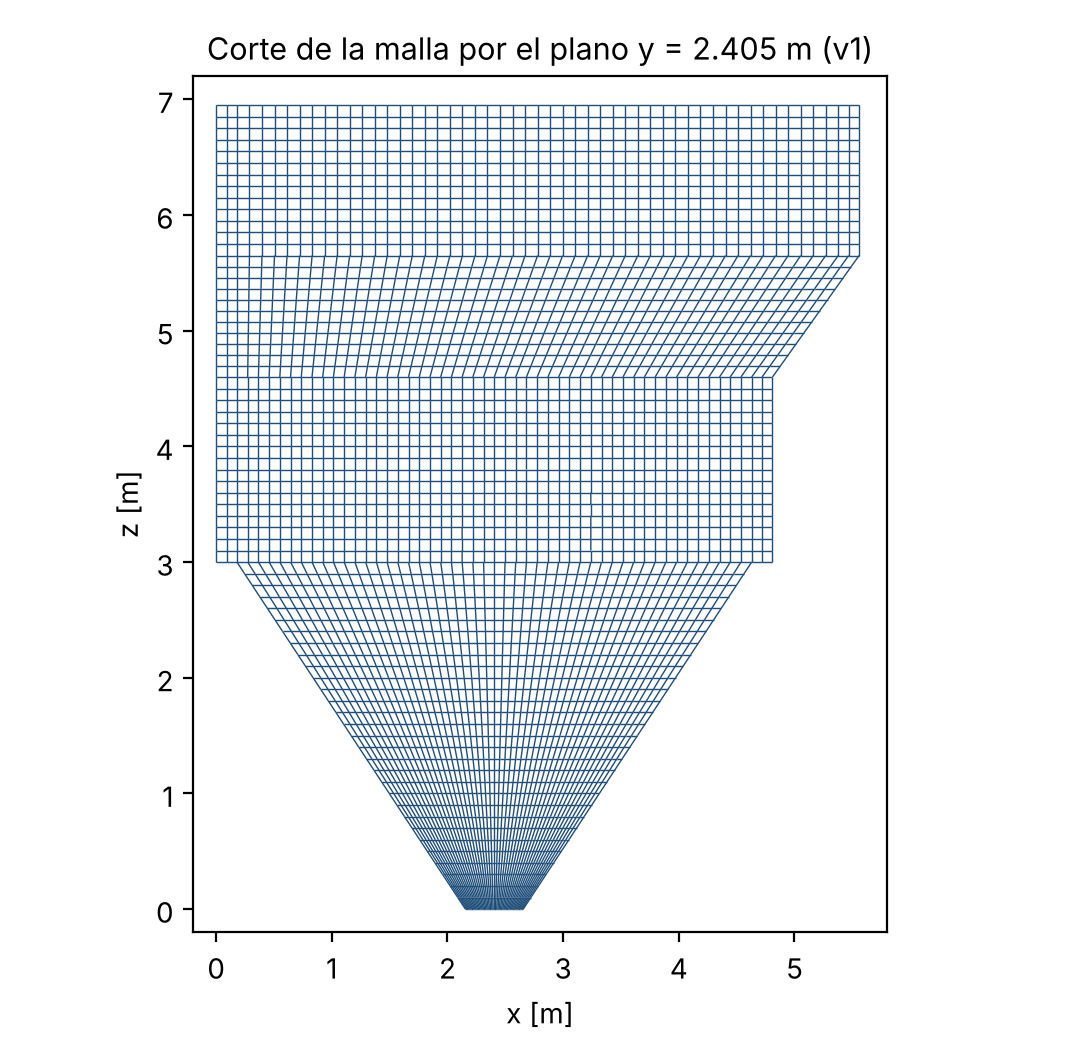
\includegraphics[width=0.46\textwidth]{fig_malla.png}
  \caption{Corte de la malla de v1 por la mitad de la pieza, $y = 2.405$ m ($x$ medido ya con el desplazamiento de 0.18 m).}
\end{figure}

Gmsh mide la calidad con \code{minSICN} (1 es un cubo perfecto). En ambas mallas las peores celdas están en el fondo de la tolva ($z < 0.5$ m), donde 0.5 m de ancho se reparten en 44 (v0) o 48 (v1) celdas de 0.01 m. En v1 esas celdas miden 0.1 m de alto (relación 10:1); la progresión 1.02 de v0 acorta la primera celda vertical a unos 0.074 m (relación 6.5:1). Conviene revisar el resultado con \code{checkMesh} (sección 7).

%---------------------------------------------------------------------
\section{Superficies y volúmenes físicos para OpenFOAM}
Los dos scripts definen dos grupos físicos, \code{internalMesh} (todas las celdas) y \code{top} (la tapa superior); el resto de las caras de borde no pertenece a ningún grupo y OpenFOAM las junta en un parche por defecto.

Un grupo físico le pone nombre a un conjunto de entidades. Por defecto Gmsh guarda en el \code{.msh} solo los elementos que están en algún grupo, y el nombre de cada \code{Physical Surface} es el que \code{gmshToFoam} usa para el parche en OpenFOAM. Si un volumen no está en ningún grupo, sus celdas no se exportan; por eso \code{internalMesh} toma todos con \code{Volume{:}}.
\begin{lstlisting}
Physical Volume("internalMesh") = {Volume{:}};

topSurface[] = Surface In BoundingBox {-1, -1, zs[5]-e, 7, 7, zs[5]+e};   // v1
Physical Surface("top") = {topSurface[]};
\end{lstlisting}
En v0 la caja es \code{{-1, -1, 6.949, 7, 7, 6.96}}, alrededor de $z = 6.95$ m.

\begin{tabularx}{\textwidth}{@{}l l l r r@{}}
\toprule
Grupo & Tipo & Entidades & Elementos v0 & Elementos v1 \\
\midrule
\code{internalMesh} & Physical Volume & 37 volúmenes & 145\,632 hexaedros & 177\,280 hexaedros \\
\code{top} & Physical Surface & 9 superficies & 2\,304 cuadriláteros & 2\,704 cuadriláteros \\
\bottomrule
\end{tabularx}

Las 9 superficies de \code{top} son la tapa del cuerpo más las tapas de las 8 franjas laterales del último tramo.

Todas las demás caras de borde (fondo y paredes de la tolva, paredes laterales y cara de aguas abajo) no están en ningún grupo físico: \code{gmshToFoam} las reúne en un parche llamado \code{defaultFaces}. Revisá su tipo en \code{constant/polyMesh/boundary} y, para un caso real, definí cada contorno con su propio grupo.

\textbf{Ejemplo para extender el caso.} El fondo de la tolva se agrega con una caja delgada alrededor de $z = 0$; en ambos scripts captura 1 superficie (1\,936 caras en v0, 2\,304 en v1).
\begin{lstlisting}
bottomSurface[] = Surface In BoundingBox {-1, -1, -0.001, 7, 7, 0.001};
Physical Surface("bottom") = {bottomSurface[]};
\end{lstlisting}
La regla es la misma para cualquier plano: una caja delgada por contorno. Las caras inclinadas (la tolva y el tramo 3) no entran en una caja delgada; se eligen con una caja que las contenga por completo o por su tag. Completá vos \code{inlet}, \code{outlet} y las paredes según el caso que quieras simular.

%---------------------------------------------------------------------
\section{Cómo ejecutar y verificar}
Del \code{.geo} al caso de OpenFOAM hay tres comandos y una revisión, y en cada paso se puede comprobar un número.
\begin{enumerate}
  \item \textbf{Mallar en formato 2.2.} \code{gmshToFoam} espera el formato 2.2 de Gmsh, y Gmsh 4 escribe por defecto uno más nuevo. En la consola deben aparecer \code{aguasArriba: 4}, \code{derecha: 12} e \code{izquierda: 12} superficies seleccionadas.
\begin{lstlisting}[language={},aboveskip=2pt]
gmsh -3 -format msh2 mallaBase3D_v1.geo -o mallaBase3D_v1.msh
\end{lstlisting}
  \item \textbf{Convertir a OpenFOAM.} Desde la carpeta del caso (la que tiene las carpetas \code{system} y \code{constant}); crea la carpeta \code{polyMesh} dentro de \code{constant}.
\begin{lstlisting}[aboveskip=2pt]
gmshToFoam mallaBase3D_v1.msh
\end{lstlisting}
  \item \textbf{Revisar \code{constant/polyMesh/boundary}.} Deben figurar los parches \code{top} y \code{defaultFaces}; ajustá el tipo de cada uno (\code{patch}, \code{wall}, etc.) antes de definir condiciones de borde en \code{0/}.
  \item \textbf{Chequear la malla.}
\begin{lstlisting}[aboveskip=2pt]
checkMesh
\end{lstlisting}
\end{enumerate}

\begin{tabularx}{\textwidth}{@{}L r r@{}}
\toprule
Qué comprobar & v0 & v1 \\
\midrule
Volúmenes geométricos en Gmsh & 37 & 37 \\
Celdas hexaédricas & 145\,632 & 177\,280 \\
Grupos físicos & \code{internalMesh}, \code{top} & \code{internalMesh}, \code{top} \\
\bottomrule
\end{tabularx}

Las unidades de la malla son metros, así que no hace falta escalarla. Si algún número no coincide, empezá por los \code{Printf}: una caja de selección que devuelve 0 superficies es la causa más frecuente.

%---------------------------------------------------------------------
\section{Comentarios}
El método A deja ver cada entidad y su número; el B es más corto y se adapta mejor cuando cambian las cotas, pero obliga a seleccionar por posición porque la numeración cambia sola.

\begin{tabularx}{\textwidth}{@{}l L L@{}}
\toprule
Criterio & A: \code{mallaBase3D_v0.geo} & B: \code{mallaBase3D_v1.geo} \\
\midrule
Extensión & 345 líneas & 103 líneas \\
Cambiar una altura & Editar varios \code{deltaV} y las cotas de las verticales & Cambiar un número de \code{zs[]} \\
Numeración de entidades & Manual y estable & Automática; cambia con \code{Coherence} y \code{Translate} \\
Resolución & Un bloque por nivel, a mano & Un bucle \code{For} sobre \code{zs[]} \\
Desplazamiento de 0.18 m & \code{x0}, \code{y0} en cada punto & Una línea \code{Translate}, con orden crítico \\
Conviene para & Entender cada paso y geometrías irregulares & Geometrías por secciones y probar cotas \\
\bottomrule
\end{tabularx}

\textbf{Errores frecuentes}
\begin{enumerate}
  \item \textbf{Caja de selección pegada al borde.} Si el límite coincide con el de la superficie, la caja devuelve 0. Dejá 0.001 m de margen y mirá el \code{Printf}.
  \item \textbf{\code{Translate} después de los \code{Transfinite}.} Se pierde la malla estructurada; ponelo justo después de \code{Coherence}.
  \item \textbf{Truncado de nodos.} \code{L / tamanoDeCelda + 1} puede dar un decimal (45.5) o quedar a una millonésima de un entero (3.9999999999999996); usá \code{Round} si querés controlar la cuenta.
  \item \textbf{Cambiar cotas sin actualizar lo demás.} En v0 el ancho (4.45), el fondo (1.975), \code{Longitud}, la altura de la tolva y las cajas de selección están escritos a mano; si cambia una cota, revisá todos. En v1 alcanza con \code{zs[]}, \code{Lx} y las secciones, pero las cajas de las extrusiones también dependen del ancho.
  \item \textbf{Tags fijos que dejan de existir.} \code{{34, 39, 44, 49}} en v1 depende de cómo numera Gmsh después de \code{Coherence} y \code{Translate}; si falla con ``Unknown OpenCASCADE entity'', revisá los tags.
  \item \textbf{\code{Layers} con decimales.} \code{celdas = 2.8} da 2 capas, no 3.
  \item \textbf{Extruir en $y$ antes que en $x$.} Las esquinas se cierran con hexaedros solo si primero se extruye en $x$: sus caras laterales entran luego en las cajas de \code{derecha} e \code{izquierda}.
\end{enumerate}

\end{document}
